\documentclass{beamer}

\usepackage[brazil]{babel}
\usepackage[alf]{abntex2cite}
\usepackage{graphicx,hyperref,uegCCETtheme,url}
\usepackage[T1]{fontenc}
\usepackage[utf8]{inputenc}
\usepackage{ragged2e}

% The title of the presentation:
%  - first a short version which is visible at the bottom of each slide;
%  - second the full title shown on the title slide;
\title[Cálculo Variacional]{Cálculo Variacional}

% Optional: a subtitle to be dispalyed on the title slide
%\subtitle{Apenas um subtítulo}

% The author(s) of the presentation:
%  - again first a short version to be displayed at the bottom;
%  - next the full list of authors, which may include contact information;
\author[Eduardo José de Oliveira]{Eduardo José de Oliveira\\Orientador: Prof. Me. Tiago de Lima Bento Pereira}

% The institute:
%  - to start the name of the university as displayed on the top of each slide
%    this can be adjusted such that you can also create a Dutch version
%  - next the institute information as displayed on the title slide
\institute[Universidade Estadual de Goiás]{
	UNIVERSIDADE ESTADUAL DE GOIÁS\\
  	Câmpus Anápolis de Ciências Exatas e Tecnológicas Henrique Santillo \\
  	Matemática}

% Add a date and possibly the name of the event to the slides
%  - again first a short version to be shown at the bottom of each slide
%  - second the full date and event name for the title slide
\date[2019]{2019}

\newtheorem{definicao}{Definição}
\newtheorem{lema}{Lema}

\newcommand{\makesubtitleframe}[1]{
	{
		\usebackgroundtemplate{
\includegraphics[width=\paperwidth]{graphics/ueg_background_title}}
		\begin{frame}
			\vfill
			\begin{center}
				{\Huge\usebeamercolor[white]{}#1}
			\end{center}
			\vfill
		\end{frame}
	}
}

\begin{document}

	\begin{frame}[plain]
	  \titlepage
	\end{frame}

\section{Objetivo}

\begin{frame}
	\frametitle{Objetivo}
	
	\justify
	O objetivo do presente trabalho é explicar o Cálculo Variacional e apresentar aplicações do mesmo.
\end{frame}

% Section titles are shown in at the top of the slides with the current section 
% highlighted. Note that the number of sections determines the size of the top 
% bar, and hence the university name and logo. If you do not add any sections 
% they will not be visible.
\section{Introdução}

\begin{frame}
	\frametitle{Introdução}
	\justify
	
  	Segundo \citeonline{calcvar}, o problema pertinente ao cálculo variacional é o de encontrar uma função diferenciável até segunda ordem $y=y(x)$ satisfazendo $y(x_1)=y_1$ e $y(x_2)=y_2$, com $x_1$, $x_2$, $y_1$ e $y_2$ dados, e $f$ uma função duas vezes diferenciável, minimizando ou maximizando a integral
	$$
		\int_{x_1}^{x_2} f(x,y,y')dx\text{.}
	$$
\end{frame}

\section{História}
\makesubtitleframe{História}

\begin{frame}
	\frametitle{Máximos e Mínimos}
	\justify
	
	Segundo \citeonline{boyer}, tem-se alguns acontecimentos importantes:
	\begin{itemize}
		\item Pierre de Fermat em 1629.
		\pause
		\begin{itemize}
			\item Comparações entre $f(x)$ e $f(x+E)$ próximo de máximos ou mínimos.
			\pause
			\item Considerar a divisão $\frac{f(x+E)-f(x)}{E}$.
			\pause
			\item Após a divisão, considerar $E=0$.
			\pause
			\item Por último, igualar o resultado a $0$, encontrando as abscissas dos máximos ou mínimos.
		\end{itemize}
		\pause
		\item Cálculo diferencial em 1665 (Isaac Newton) e 1676 (Gottfried Leibniz).
	\end{itemize}
\end{frame}

\begin{frame}
	\frametitle{Problema da Braquistócrona}
	\justify
	
	Segundo \citeonline{hist_courant} e \citeonline{hist_still}, o problema da braquistócrona,
	\begin{itemize}
		\item Foi formulado por Johann Bernoulli em 1969 e pode ser apresentado como:
		\begin{block}{Problema da Braquistócrona}
			Sejam $A$ e $B$ dois pontos dados em um plano vertical. O problema da braquistócrona consiste em encontrar a curva que uma partícula M precisa descrever para sair de A e chegar em B no menor tempo possível, somente sob a ação da força da gravidade \cite[p. 3]{calcvar}.
		\end{block}
	\end{itemize}
\end{frame}

\begin{frame}
	\frametitle{Problema da Braquistócrona}
	\justify

	Segundo \citeonline{hist_courant} e \citeonline{hist_still},
	\begin{itemize}
		\item A Solução de Jacob Bernoulli (1697) apresenta o aspecto da curva variável.
		\pause
		
		\item Euler e Lagrange.
	\end{itemize}
\end{frame}

\section{Cálculo Variacional}
\makesubtitleframe{Cálculo Variacional}

\begin{frame}
	\frametitle{Relembrando o problema}
	\justify
	
	Deseja-se, no Cálculo Variacional, encontrar uma função diferenciável até segunda ordem $y=y(x)$ satisfazendo $y(x_1)=y_1$ e $y(x_2)=y_2$, com $x_1$, $x_2$, $y_1$ e $y_2$ dados, e $f$ uma função duas vezes diferenciável, minimizando ou maximizando a integral
	\begin{equation}
		\int_{x_1}^{x_2} f(x,y,y')dx\text{.}
		\label{eqn:def_calcvar}
	\end{equation}
\end{frame}

\begin{frame}
	\frametitle{Funções Aproximadoras}
	\begin{definicao}
		\justify
		Uma família de funções aproximadoras é definida como
		$$Y(x)=y(x)+\varepsilon \eta (x)\text{,}$$
		onde a função $\eta (x)$ é uma função diferenciável arbitrária para a qual $\eta (x_1)=\eta (x_2)=0$. O número $\varepsilon$ é o parâmetro da família. Sua derivada pode ser escrita como
		$$Y'(x)=y'(x)+\varepsilon \eta '(x)\text{.}$$
	\end{definicao}
\end{frame}

{
	\usebackgroundtemplate{}
	\begin{frame}
		\begin{figure}
			\caption{Representação gráfica das funções aproximadoras.}
			\begin{center}
				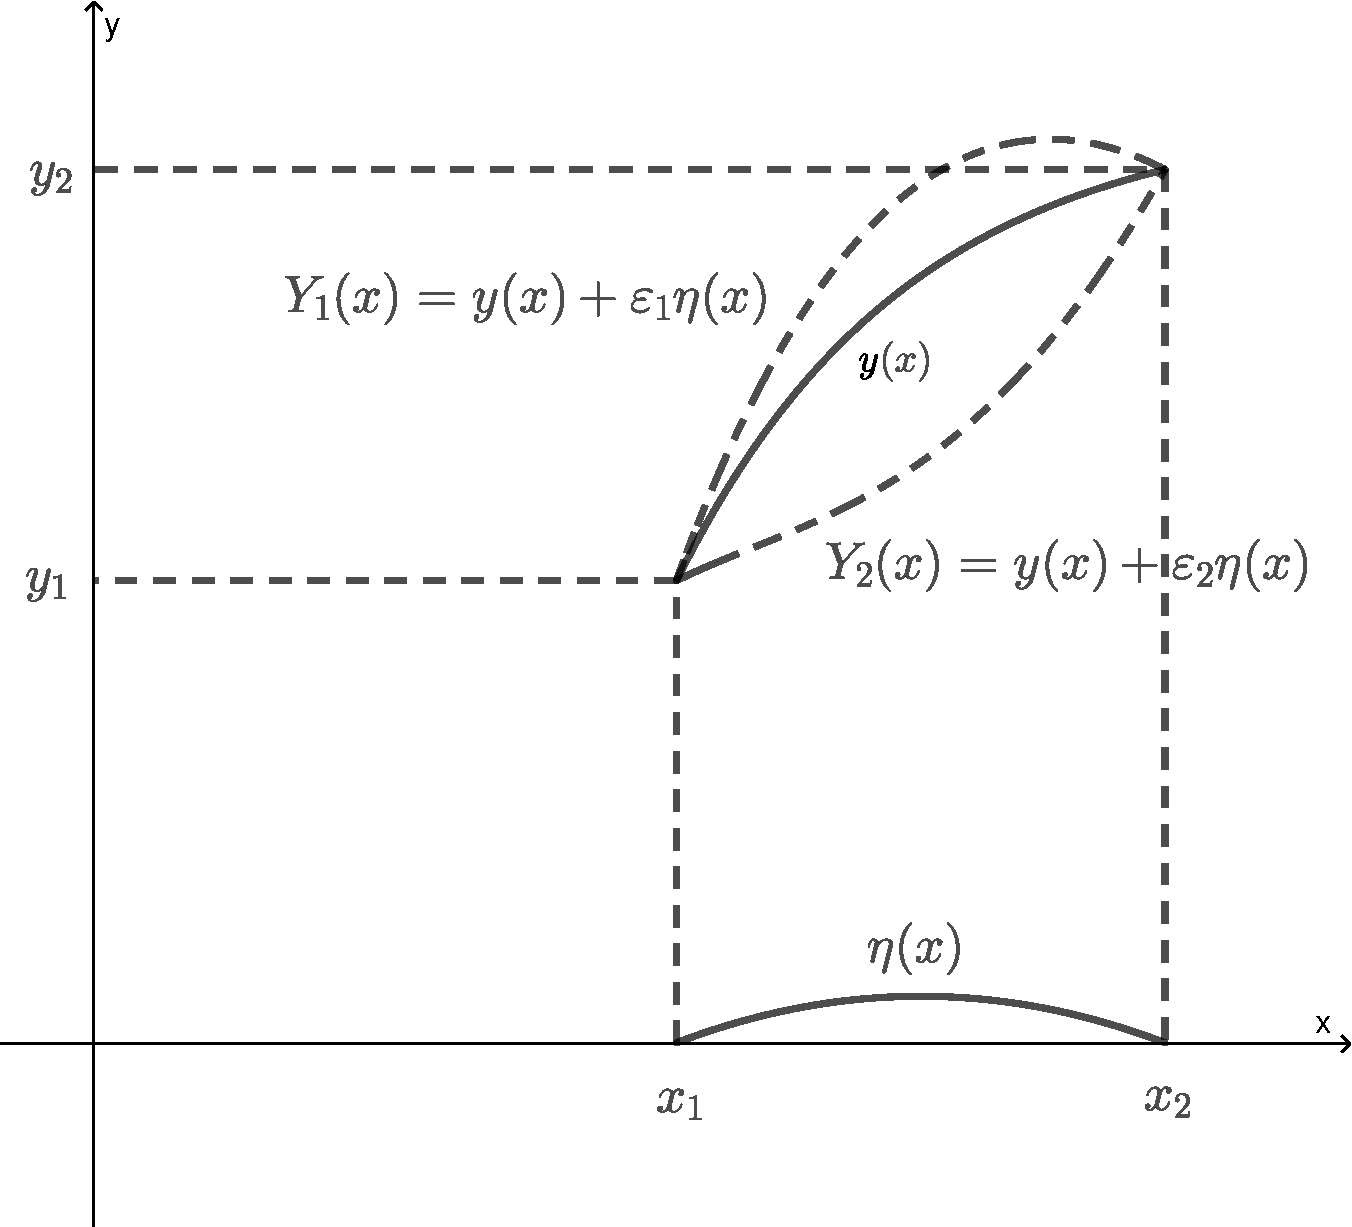
\includegraphics[scale=0.25]{../figuras/cap_calcvar/figura_001}\par
				{\small Fonte: Elaborada pelo autor, 2019}
			\end{center}
			\label{fig:func_approx}
		\end{figure}
	\end{frame}
}
	
\begin{frame}
	\frametitle{Reescrevendo o Problema}
	\justify
	
	Pode-se reescrever a integral \eqref{eqn:def_calcvar} utilizando as funções aproximadoras, dependendo de $\varepsilon$, então
	\begin{equation}
		\label{eqn:int_funcional_approx}
		I(\varepsilon)=\int_{x_1}^{x_2}f(x, Y, Y')dx\text{.}
	\end{equation}
	
	Para encontrar a função $y(x)$ que maximiza ou minimiza a integral escrita com as funções aproximadoras \eqref{eqn:int_funcional_approx}, deve-se fazer
	$$I'(\varepsilon)=0\text{,}$$
	e, considerando que quando $\varepsilon=0$, as integrais \eqref{eqn:def_calcvar} e \eqref{eqn:int_funcional_approx} fornecem os mesmos maximos e mínimos, é necessário que
	$$I'(0)=0\text{.}$$
\end{frame}

\begin{frame}
	\justify
	
	Utilizando a Regra de Leibniz, pode-se escrever a derivada de $I(\varepsilon)$ como
	$$I'(\varepsilon)=\int_{x_1}^{x_2} \frac{\partial f}{\partial \varepsilon} (x, Y, Y') dx \text{,}$$
	\pause
	donde, aplicando a regra da cadeia, obtêm-se
	$$I'(\varepsilon)=\int_{x_1}^{x_2}\left ( \frac{\partial f}{\partial x}\frac{\partial x}{\partial \varepsilon} + \frac{\partial f}{\partial Y} \frac{\partial Y}{\partial \varepsilon} + \frac{\partial f}{\partial Y'} \frac{\partial Y'}{\partial \varepsilon} \right )dx\text{.}$$
	\pause
	
	O primeiro termo do integrando é nulo, pois $x$ independe de $\varepsilon$, então
	$$
		I'(\varepsilon)=\int_{x_1}^{x_2}\left ( \frac{\partial f}{\partial Y}\frac{\partial Y}{\partial \varepsilon} + \frac{\partial f}{\partial Y'}\frac{\partial Y'}{\partial \varepsilon} \right ) dx \text{.}
	$$
\end{frame}

\begin{frame}
	\justify
	
	Derivando a função aproximadora $Y(x)=y(x)+\varepsilon \eta(x)$ em relação a $\varepsilon$, conclui-se que
	$$\frac{\partial Y}{\partial \varepsilon}=\eta\text{.}$$
	\pause
	
	De modo análogo, ao derivar $Y'(x)=y'(x)+\varepsilon \eta '(x)$ em relação a $\varepsilon$, obtêm-se que
	$$\frac{\partial Y'}{\partial \varepsilon}=\eta '\text{.}$$
\end{frame}

\begin{frame}
	\justify
	
	Substituindo $\frac{\partial Y}{\partial \varepsilon}=\eta$ e $\frac{\partial Y'}{\partial \varepsilon}=\eta'$ em $I'(\varepsilon)$,
	$$
		I'(\varepsilon)=\int_{x_1}^{x_2}\left ( \frac{\partial f}{\partial Y}\frac{\partial Y}{\partial \varepsilon} + \frac{\partial f}{\partial Y'}\frac{\partial Y'}{\partial \varepsilon} \right ) dx
	$$
	\pause
	$$
		I'(\varepsilon)=\int_{x_1}^{x_2}\left ( 
			\frac{\partial f}{\partial Y} \eta +
			\frac{\partial f}{\partial Y'} \eta '
		\right )dx \text{.}
	$$
\end{frame}

\begin{frame}
	\justify
	
	Calculando $I'(0)$, ou seja, quando $\varepsilon=0$, é possível trocar $Y$ e $Y'$ por $y$ e $y'$, respectivamente, então,
	$$
		I'(0)=\int_{x_1}^{x_2}\left (
			\frac{\partial f}{\partial y} \eta +
			\frac{\partial f}{\partial y'} \eta '
		\right )dx
	$$
	\pause
	$$
		I'(0)=
			\int_{x_1}^{x_2} \frac{\partial f}{\partial y}\eta dx
			+
			\int_{x_1}^{x_2} \frac{\partial f}{\partial y'}\eta' dx \text{.}
	$$
	\pause
	
	Integrando o segundo membro por partes, tem-se
	$$
	I'(0)=
		\int_{x_1}^{x_2} \frac{\partial f}{\partial y}\eta dx
		-
		\int_{x_1}^{x_2} \frac{d}{dx} \left ( \frac{\partial f}{\partial y'} \right ) \eta dx
	$$
\end{frame}

\begin{frame}
	\justify
	
	Organizando $I'(0)$, tem-se
	$$
		I'(0)=\int_{x_1}^{x_2}\left (
			\frac{\partial f}{\partial y} -
			\frac{d}{dx}
			\left (
				\frac{\partial f}{\partial y'}
			\right )
		\right )\eta dx
		\text{.}
	$$
	\pause
	
	Devido a condição necessária, $I'(0)=0$, escrevemos
	$$
		I'(0)=\int_{x_1}^{x_2}\left (
			\frac{\partial f}{\partial y} -
			\frac{d}{dx}
			\left (
				\frac{\partial f}{\partial y'}
			\right )
		\right )\eta dx = 0
		\text{.}
	$$
\end{frame}

\begin{frame}
	\justify
	Para concluirmos a dedução do resultado é necessário o uso do seguinte lema:
	
	\begin{lema}
		\justify
		Sejam $x_1 < x_2$ fixos e $G(x)$ uma função contínua particular para $x_1 \leqslant x \leqslant x_2$. Se $$\int_{x_1}^{x_2} \eta (x) G(x) dx = 0$$ para cada função diferenciável $\eta (x)$ tal que $\eta (x_1)=\eta (x_2)=0$, concluímos que $G(x)=0$, para todo $x$ de modo que $x_1 \leqslant x \leqslant x_2$.
	\end{lema}	
	
\end{frame}

\begin{frame}
	\frametitle{Equação de Euler-Lagrange}
	\justify
	
	Pelo Lema anterior, conlui-se que
	$$
		\frac{\partial f}{\partial y} - \frac{d}{dx} \left ( \frac{\partial f}{\partial y'} \right )=0 \text{.}
	$$
	\pause
	
	A equação acima é chamada de \textbf{Equação de Euler-Lagrange}, sendo uma condição necessária para minimizar ou maximizar a integral
	$$
		\int_{x_1}^{x_2} f(x, y, y')dx \text{.}
	$$
\end{frame}

\section{Referências}
\begin{frame}
	\frametitle{Referências}
	\bibliography{../references}
\end{frame}

\end{document}
